\documentclass{llncs}
\RequirePackage[T1]{fontenc}
\usepackage[cp1250]{inputenc}

\usepackage{pgf}
\usepackage{tikz}
\usepackage{listings}
\usepackage{url}
\usepackage{xspace}
%\numberofauthors{3}
\author{
%\alignauthor
J�drzej Fulara and
%\affaddr{Institute of Informatics}\\
%\affaddr{University of Warsaw}\\
%\affaddr{ul. Banacha 2}\\
%\affaddr{02-097 Warsaw, Poland}\\
%\email{fulara@mimuw.edu.pl}
%\alignauthor
Krzysztof Jakubczyk and
%\affaddr{Institute of Informatics}\\
%\affaddr{University of Warsaw}\\
%\affaddr{ul. Banacha 2}\\
%\affaddr{02-097 Warsaw, Poland}\\
%\email{kjk@mimuw.edu.pl}
%\alignauthor
Aleksy Schubert
%\affaddr{Institute of Informatics}\\
%\affaddr{University of Warsaw}\\
%\affaddr{ul. Banacha 2}\\
%\affaddr{02-097 Warsaw, Poland}\\
%\email{alx@mimuw.edu.pl}
}
\bibliographystyle{abbrv}
\title{Supplementing Java Bytecode with Specifications}
\institute{%
Institute of Informatics\\
University of Warsaw\\
ul. Banacha 2\\
02-097 Warsaw, Poland}



\newcommand{\jmltobmltext}{JML2BML}
\newcommand{\jmltobml}{\textsl{\jmltobmltext}\xspace}
\newcommand{\openjml}{OpenJML\xspace}
\newcommand{\bmllib}{BMLLib\xspace}
\newcommand{\hs}{\hspace{0.5pt}}




\lstdefinelanguage{BML}{morekeywords={abstract,break,byte,case,catch,char,class,%
      const,continue,default,do,double,else,extends,false,final,%
      finally,float,for,goto,if,implements,import,instanceof,%
      interface,label,long,native,new,
      boolean, int,%
      null,%
      package,private,protected,public,ghost,%
      return,short,static,super,switch,synchronized,this,throw,%
      throws,transient,true,try,void,volatile,while,
      requires,precondition,ensures,exsures,exists,forall,&&,%
      old_this,loop_inv,\result,\everything,\nothing,%
      loop_specification,modifies,invariant,decreases,%
      iconst_0,iconst_1,istore_3,iinc,iload_3,%
      aaload,aload_0,aload_1,aload_2,aastore,%
      if_acmpne,if_icmplt,%
      invokespecial,getfield,%
      arraylength,ireturn},%
   sensitive,%
   morecomment=[l]//,%
   morestring=[b]",%
   morestring=[b]',%
    basicstyle=\scriptsize,
    keywordstyle=\bfseries\color{black},
    commentstyle=\itshape\color{blue},
    mathescape=true,
}


\begin{document}
\maketitle


%\section{What should be in paper}
%\begin{itemize}
%	\item What is JML
%	\item What is BML
%	\item Why is translation needed??
% \item Why the tool needed?? (JVM -> VM) BML can be used to different languages, JML to one??
%	\item The tool isn't built on any existing comipler.
%	\item As input we get source file with JML annotations and compiled class file.
%	\item Therefore we can't used optimised bytecode (problem with loops, assertions etc.)
%	\item Optimized bytecode may be used for more general annotations eg. method invariants.
%	\item Detecting loops in bytecode
%	\item Description of matching source code with bytecode loops
%	\item Non-trivial example
%\end{itemize}
%\maketitle

\begin{abstract}
  The proof-carrying code (PCC) techniques allow the executable code
  to be augmented with a proof that the code obeys certain policies
  (e.g. the program does not store passwords in clear in a file). BML
  (Bytecode Modeling Language) can be regarded as a part of the PCC
  architecture which allows expressing detailed properties of Java
  bytecode programs.  As most of the programming is done at the source
  code level, it is desirable to have a way to translate properties
  expressed at the source code level (in our case written in Java
  Modeling Language, JML) to the bytecode level.  In this paper we
  present a \jmltobml compiler, a tool that for a given Java source
  file annotated with specifications generates class files with BML.\\[0.5\baselineskip]

  {\bf Keywords:} formal methods, proof carrying-code, Java bytecode
\end{abstract}

%# Alternative languages on the Java VM
%# Java Extensions
%#  - PCC
%#  Optimization
%#  - PCC
%# VM Design
%# Java Verification
%#  - PCC
%#Java for Embedded Systems
%*   Middleware for Mobile Applications
%* Location-Based Services
%* M-Business Applications
% page limit: 10 pages

%\category{D.2.4}{Software Engineering}{Software/Program Verification}

%\terms{Reliability, Verification}

%\keywords{Java, bytecode, JML, BML} % NOT required for Proceedings

\section{Introduction}

The bytecode verification process performed by Java Virtual Machine
(JVM) ensures vital properties of programs such as that all operand
arguments on the operand stack are correct legal, there are enough
arguments on the stack etc.  In certain situations, these guarantees
are not sufficient. In particular, many of the security guarantees are
ensured at runtime. For instance, a mobile application asks the user
to acknowledge the sending of data over the mobile network. However,
the user may get bored with many such prompts and disable this
security feature. After this, she or he may easily be made to send
data to e.g. an expensive premium number. It would be more secure to
give the user a load- (or download-) time guarantee that the code
sends data only to expected receivers.  Currently, this is partially
done through digital certificates. The certificates, however, do not
assure that the software is indeed safe. They only certify who takes
(not so well defined) responsibility for the problems caused by the
program.  In fact, there were cases that a signed code caused serious
security problems~\cite{BMGcase}.

Another guarantee which is not assured by the traditional bytecode
verification procedure is the lack of code flaws such as occurrences
of null-pointer exceptions, array index out of bounds exceptions
etc. In many cases, these flaws can be eliminated with the help of
some additional information, e.g. @NonNull annotations, suggested
in~\cite{JSR305} (much in the way non-termination can be eliminated
with help of the number of steps the underlying machine can
take). Additionally, if the extended verification procedure would
verify the lack of null-pointer exceptions then the checks for null
values could be eliminated from the execution of bytecode instructions
which would give a performance boost.

The goal of the proof-carrying code (PCC)
technique~\cite{pcc} is to give the user certain guarantees of the
code to be executed at the moment of its execution. The check of the expected policy is performed by the user (or by the user's execution environment) before the code is executed (see
Fig.~\ref{fig:pccScheme}).

\begin{figure}
\begin{center}
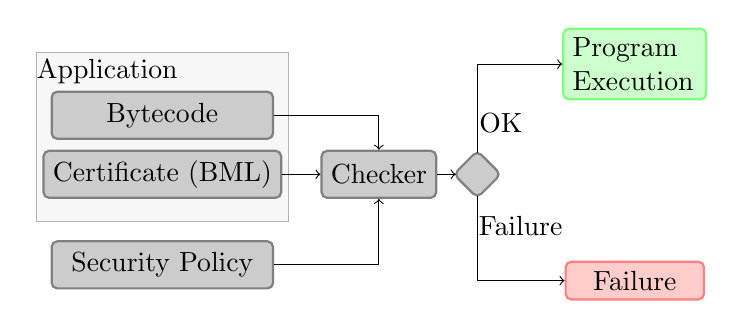
\begin{tikzpicture}[scale=0.5]

\tikzstyle{vertex}=[rectangle,draw=black!50,fill=black!20,thick,rounded corners = 2pt, minimum width=80pt, minimum height=17pt]
\tikzstyle{vertex2}=[rectangle,draw=black!50,fill=black!20,thick,rounded corners = 2pt, minimum height=17pt]
\tikzstyle{vertex3}=[rectangle,draw=green!50,fill=green!20,thick,rounded corners = 2pt, minimum width=50pt, text width=45pt]
\tikzstyle{vertex4}=[rectangle,draw=red!50,fill=red!20,thick,rounded corners = 2pt, minimum width=50pt]

\tikzstyle{rotated}=[rectangle,draw=black!50,fill=black!20,thick,rounded corners = 2pt,rotate=45, minimum height=12pt, minimum width = 12pt]
\tikzstyle{rl}=[line join = round]
\filldraw[draw=black!30,fill=black!3] (-3.2,3.8) rectangle (3.2,-0.5);
\node (app) at(-1.4,3.3) {Application};
\node[vertex] (bytecode) at (0,2.2){Bytecode};
\node[vertex] (certificate) at (0,0.7) {Certificate (BML)};

\node[vertex](policy) at (0, -1.6) {Security Policy};

\node[vertex2](checker) at (5.5,0.7) {Checker};
\node[rotated](rot) at (8, 0.7) {};
\node[vertex3](execution) at (12,3.5) {Program Execution};
\node[vertex4](failure) at (12,-2) {Failure};
\draw[->] (certificate) to[out=0,in=180] (checker);
\draw[->] (checker.east) -- (7.45,0.7);
\draw[->] (bytecode.east) -- (5.5,2.2) -- (checker.north);
\draw[->] (policy.east) -- (5.5,-1.6) -- (checker.south);
\draw[->] (8,1.25) -- (8,3.5) -- (execution.west);
\draw[->] (8,0.15) -- (8,-2) -- (failure.west);
\node (ok) at (8.6, 2) {OK};
\node (ok) at (9.1, -0.6) {Failure};
\end{tikzpicture}
\end{center}
\caption{Proof-Carrying Code architecture for bytecode}
\label{fig:pccScheme}
\end{figure}



One of the possible ways to realise the PCC architecture is developed
under the European project MOBIUS.\footnote{See
\url{http://mobius.inria.fr}} The logic-based methods developed in the project
\cite{MOBIUSscenarios} rely on specification
of object-oriented code in the fashion governed by the
design-by-contract principles~\cite{DesignByContract}. Bytecode
Modeling Language (BML) is a specification language which realises the
methodology at the bytecode level~\cite{bmlBurdy}. It is designed as a
counterpart of the Java Modeling Language (JML), an established
specification language dedicated to formally describe properties of
Java programs in the design-by-contract style~\cite{JML}.

Multiple languages can now be compiled to the Java bytecode: Python,
JavaScript, Scala, etc.  At SugarCon 2008, Sun Microsystems President
and CEO Jonathan Schwartz said "we are just going to take the 'J' off
the 'JVM' and just make it a 'VM'". Therefore there will be a global
trend with support of companies to use JVM with languages other than
Java.  It is, thus, important to be able to express specifications at
the bytecode level\hs{}---\hs{}in case the development is done in many
languages the only common platform is the platform of the executable
code. This explains the efforts concerning BML specification language.

The JML specification language exists already for several years. A lot of code has been annotated with the
specifications in this language (see~\cite{overviewOfJML} for an
overview). Except for that, it is easier to understand and specify the
code in the source form than in the bytecode form. In this light, it
is desirable to be able to translate these specifications from JML to
BML. Moreover, the code producer in PCC scenarios, who has to produce
a correctness proof, will often prefer to construct it in terms
of the source code rather than in terms of the bytecode, and then compile the
specification and the proof into the level of executable code.

In a broader perspective, the full infrastructure to support the use
of BML annotated programs, for which complicated properties are
checked at the user's end, requires the following items:
\begin{itemize}
\item PCC checker tools for BML annotations combined with
  PCC certificates,
\item tools which enable the construction of PCC certificates,
\item procedures to safely distribute the desired properties to be
  checked by PCC infrastructure,
\item modeling languages (such as JML) for other programming
  languages,
\item compilers that transform programs to JVM bytecode with
  annotations.
\end{itemize}
The \jmltobml compiler described in this paper is designed to be a
part of this scheme which translates the policies and specifications
to the bytecode format.


\paragraph{Organisation of the paper}
In Sect.~\ref{sec:specification}, we present specification
languages JML and BML. An example which illustrates the work of the
compiler is presented in Sect.~\ref{sec:example}.
Sect.~\ref{sec:compiler} overviews the design of the \jmltobml
compiler. The problem of placing BML annotations in the bytecode is discussed in Sect.~\ref{sec:loops}. Related work is presented in
Sect.~\ref{sec:related-work}.


\section{Specification languages}
\label{sec:specification}


\subsection{JML}
The Java Modeling Language (JML) is a behavioural specification
language for Java programs~\cite{JML}. It allows writing
specifications in the \textit{design-by-contract}
fashion~\cite{DesignByContract}. Data types and method behaviour can
be precisely documented using JML annotations. They describe
invariant properties that are maintained by objects, input method
requirements (preconditions), what we can expect at the output of
the method (postconditions) and also some lower level properties of the
code (such as loop invariants). JML annotations are written in
standard Java comments, so they do not disturb standard Java
compilers.

The software development process must be divided into implementation
and integration of multiple smaller components.  JML allows to
precisely specify desired behaviour of the components which is
crucial in case they must be combined with as little implementers'
intervention as possible~\cite{SoftwareReuse}. JML is also a language
which abstracts from implementation details. Therefore it
can be used to document \emph{what} is written in code,
but to hide \emph{how} it is done. Moreover, it makes possible to
automatically check that the documentation up to date~\cite{formalDocumentation}.

JML stays as close as possible to the Java syntax and semantics to 
ensure the readability of its specifications and its tool support
is rich (see~\cite{overviewOfJML}). In
particular, there are tools that check JML specification at
runtime~\cite{runtime}, in extended static checking
fashion~\cite{escJava}, and allow to perform software
certification~\cite{krakatoa}. There are also tools that support
annotation generation~\cite{canapa,daikon}.


\subsection{BML}


The Bytecode Modeling Language (BML) is a specification language for
Java bytecode. It was proposed by Burdy et al. in~\cite{bmlBurdy}.\
The
design of BML directly follows the fundamental concepts of JML. It
inherits most constructions and keywords from the JML syntax. As 
BML is developed within the MOBIUS~\cite{mobius} project and the main
target of the project are Java-enabled mobile devices such as mobile
phones, the current version of BML assumes some simplifications of the
Java bytecode which are present in the J2ME mobile platform.

Class files with BML annotations are regular Java class files,
executable by all Java tools. The annotations are stored within
additional attributes. The BML related attributes start with the
prefix \texttt{org.bmlspecs} and according to the specification of JVM
they should be ignored in normal execution, since their names are not part
of the original JVM specification.

Following the logical structure of class files, class
specifications are stored as class attributes, method specifications,
as method attributes and specifications inserted in
the bytecode are subattributes of the JVM Code attributes.


\subsection{Overview of annotations}


The structure of annotations in BML and JML is very similar. We have
two main types of annotations: method annotations and data type (class
and interfaces) annotations.


\subsubsection{Method annotations}
The most important type of method annotations are \textit{method
specifications} which describe the input-output behaviour of the
method. These are preconditions (\texttt{requires}), defining
conditions that should be fulfilled before entering the method and
postconditions (\texttt{ensures}) telling what we can expect after the
method finishes. One can define also which fields are modified (clause
\texttt{modifies}) and which exceptions might be thrown (clause
\texttt{signals}).

The other type of method annotations are specifications 
appearing between mnemonics, such as:
\begin{itemize}
\item {Assert clauses which state some facts about fields,
  variables etc. that should hold at this point of program execution.}
\item {Loop specifications that describe loop invariants
    (\texttt{loop\_invariant}), loop termination measures
    (\texttt{decreases}), and modification scopes (\texttt{modifies}).}
\item {Declarations of local \texttt{ghost}
  variables\hs{}---\hs{}variables that are visible only in the
  specifications and that can be modified only using special
  \texttt{set} instructions.}
\item {\texttt{Set} instructions are similar to Java assignments, but
  they operate on ghost fields and variables.}
\end{itemize}


\subsubsection{Data type annotations}
Class (and interface) specifications describe the behaviour of a class
as a whole (in the \texttt{static} version) or of objects
(\texttt{instance}). The most important type of \textit{class
specifications} are class invariants. They describe the property that
should hold for all objects of this class in all \textit{visible}
states, i.e. after all constructors and before and after all
methods. For example, having a field \texttt{Object[] list}, one can
write an invariant that the list is never null and its length is
10. Class invariants can be seen as additional, implicit preconditions
and postconditions for all methods in the class.

Other important class specifications are declarations of \texttt{ghost} and \texttt{model} fields. Ghost fields are similar to
  local ghost variables, but are visible in the whole class scope. Model fields are present only in the specifications,
  representing some more complicated formulae. For example one can
  create a model field representing the property that a collection does
  not contain nulls.
More details can be found in~\cite{jmlrefman} and~\cite{bmlrefman}.

\lstset{language=java, morekeywords={requires,ensures,\result,\exists,\old,loop_invariant,\forall,==>, decreases},
        basicstyle=\scriptsize,commentstyle=\scriptsize,moredelim=*[s][\scriptsize]{/*@}{*/},
        numbers=left,numberstyle=\tiny,stepnumber=4,numbersep=5pt}
\begin{figure}[htbp]
~\hspace{2cm}\begin{minipage}{400pt}
\begin{lstlisting}
public class List {

  private Object[] list;

  /*@ requires list != null;
    @ ensures \result ==(\exists int i;
    @ 0 <= i && i < list.length &&
    @ \old(list[i]) == o1 && list[i] == o2);
    @*/
  public boolean replace(Object o1, Object o2){
    /*@
      @ loop_invariant i <= list.length
      @ && i >=0 && (\forall int k;0 <= k
      @ && k < i ==> list[k] != o1);
      @ decreases list.length - i;
      @*/
    for (int i = 0; i < list.length; i++) {
      if (list[i] == o1) {
        list[i] = o2;
        return true;
      }
    }
    return false;
  }
}
\end{lstlisting}
\end{minipage}
\caption{An example class \texttt{List.java} containing single method
\texttt{replace}}
\label{fig:source}
\end{figure}


\section{An example of using the compiler}
\label{sec:example}


\subsection{Source code}

Consider the class presented on Fig.~\ref{fig:source}. This is an
excerpt of a class which implements a sequence of objects. We present
here only one method that replaces in the \texttt{list} array the
first occurrence of its first parameter with the second one. True will
be returned, if and only if such an element was found.

The presented code, apart from standard Java statements, contains also
specifications in JML. There is a precondition (\texttt{requires ...})
for the method \texttt{replace} defined. It requests that every time
the method is invoked, the field \texttt{list} is not
\texttt{null}\footnote{In general a method can have multiple
  \texttt{requires-ensures} pairs. In this case the method can be
  invoked only in places where a condition specified by at least one
  of the \texttt{requires} clauses holds.}. The next three lines
(starting with \texttt{ensures}) are the method
postcondition. It states that, if the precondition was fulfilled, then
the method result is true if and only if there was an element in the
\texttt{list} the value of which has been updated from \texttt{o1} to
\texttt{o2}. This is the guarantee which is ensured by the method
call.  Note that the postcondition uses the JML primitives
such as \texttt{$\backslash$result}, \texttt{$\backslash$old} or
\texttt{$\backslash$exists}. This postcondition does not describe all
desirable properties of this method. For example an implementation that replaces
all elements in the \texttt{list} up to the first occurrence of
\texttt{o1} with \texttt{o2} will fulfil this specification.
\begin{figure}[htb]
\lstset{language=bml}
\lstset{basicstyle=\scriptsize,stepnumber=400,numbersep=5pt}
\vspace{-2\baselineskip}
~\hspace{2cm}~\begin{minipage}{400pt}
\begin{lstlisting}
/*@
  @ requires this.list != null
  @ ensures \result ==
  @   (\exists int i; 0 <= i &&
  @            i < this.list.length &&
  @            old_this.list[i] == o1 &&
  @            this.list[i] == o2)
  @*/
public boolean replace(Object o1, Object o2)
0:    iconst_0
1:    istore_3
2:    goto	   #27
5:    aload_0
6:    getfield	   main.List.list
9:    iload_3
10:   aaload
11:   aload_1
12:   if_acmpne	   #24
15:   aload_0
16:   getfield	   main.List.list
19:   iload_3
20:   aload_2
21:   aastore
22:   iconst_1
23:   ireturn
24:   iinc	   %3	1
27:   iload_3
28:   aload_0
29:   getfield	   main.List.list
32:   arraylength
/*@
  @ loop_specification
  @   modifies everything
  @   invariant i <= this.list.length &&
  @      i >= 0 &&
  @      (\forall int k; 0 <= k &&
  @          k < i ==> this.list[k] != o1)
  @   decreases this.list.length - i
  @*/
33:   if_icmplt	   #5
36:   iconst_0
37:   ireturn
\end{lstlisting}
\end{minipage}


\caption{The method \texttt{replace} in the \texttt{List.class}}
\label{fig:bytecode}
\end{figure}


In addition to the specification of the input-output beha\-viour of
the method, also the main loop of the \texttt{replace} method is
annotated. The \texttt{loop\_invariant} clause contains the invariant:
a formula that holds at the beginning of the loop body at each
loop iteration. In this example it states that in iteration \texttt{i}
there are no occurrences of \texttt{o1} in \texttt{list} on positions
before \texttt{i}. The annotation \texttt{decreases} describes the
loop variant. It gives an expression (in this case
\verb|list.length - i|) the value of which is decreased in each loop
iteration by at least one.

\subsection{Bytecode}

In this section we describe the result of translating the source code
from Fig.~\ref{fig:source}. The actual result  is
a class file enriched with attributes which contain the
representation of BML specifications. However, binary class
files are not human readable. Thus, we rely for the 
presentation on its textual representation obtained from Umbra
\cite{bmllib}. Fig.~\ref{fig:bytecode} shows the translated
\texttt{replace} method together with BML annotations inserted by our
\jmltobml compiler. The bytecode instructions labelled with 0 and 1
correspond to the initialisation \texttt{i = 0}. The loop is located
between lines 2 and 33. Lines 5--12 represent the \texttt{if}
statement, 15--23 correspond to lines 19--20 from the source
code. Loading loop condition parameters is located in lines 27--32 and
33 performs the loop condition comparison.

The JML \texttt{requires-ensures} pair is directly translated to a
corresponding \texttt{requires-ensures} pair at the BML level. We can
see that the translation is almost literal copy of the original
formula. The only difference is in the way the objects are referenced
(BML requires to add an explicit \texttt{this} prefix to fields) and the
\texttt{$\backslash$old} operator becomes a part of the \texttt{this}
reference).

Loop specifications are located after the line labelled with~32 in the
presented listing. The \jmltobml compiler detects loops in the
bytecode and inserts the annotation before the bytecode representing
the final conditional jump. In this case it is the \texttt{if\_icmplt}
instruction comparing \texttt{i} and \texttt{list.length} (detecting
loops is described in Sect.~\ref{sec:loops}.) The modifies clause
describes a set of variables modified by the loop. We can see it in
the listing as this clause is obligatory in BML. Currently, because of
\openjml limitations, it is not supported by our compiler so we see
the default value (\texttt{everything}) inserted at this point.


\section{\jmltobmltext{} compiler design}
\label{sec:compiler}

The \jmltobml takes as an input a Java source file with JML annotations
together with the corresponding class file and outputs the class file
with proper BML annotations inserted. Our compiler uses an enhanced
Abstract Syntax Tree (AST) for the Java source code, taken from the
\openjml\footnote{Available from
\url{http://sourceforge.net/projects/jmlspecs}} compiler (a Java
compiler with JML checker based upon OpenJDK). For
different types of JML clauses, there are separate translation rules
defined. At each node of the AST, all translation rules are
applied. If some rule succeeds to translate this node, the result is
stored in the class file, using the \bmllib
library~\cite{bmllib}. This approach makes the compiler easily extensible. It
is enough to just write a new translation rule to support additional
features of the JML language. Moreover, the acyclic structure of the
code should make the future maintenance more feasible and facilitate
the understanding of the code mechanisms by future
contributors~\cite{Dijkstra70}.



Currently, the \jmltobml compiler focuses on a subset of JML
called JML Level 0~\cite[Sect. 2.9]{jmlrefman}. Due to external
libraries limitations not all desired features are translated, for
example the loop \texttt{modifies} clause is not supported by
\openjml. The \jmltobml compiler is designed to be compatible with
other bytecode level tools, such as the bytecode editor
\textit{Umbra}.


\subsection{Translation mechanism}

\subsubsection{Translation rules}
The \jmltobml compiler uses a set of translation rules, each
responsible for a relatively small, independent piece of
translation. For example we have a separate rule for translating
assert and another one for translating loop invariant. Each rule is responsible for translation of
a part of the AST tree resulting from a particular non-terminal of the
input grammar (in most cases it boils down to the situation that each
rule is applied exactly to one AST node). Translation rule may write
results of the translation to the output class file (using \bmllib). It
can, however, only collect some translated data that may be used by
other translation rules. For example both\hs{}---\hs{}the
\texttt{assert} and \texttt{loop\_invariant} annotations contain
expressions. Therefore we created an expression translation rule that does not write anything to the
output file\hs{}---\hs{}just returns the translated expression that
will be used in other translation rules.

It is relatively easy to extend the translation using the translation rule
concept. One simply provides a new implementation of a translation rule and registers it in the manager.
Translation rule key design features are:
\begin{itemize}
\item the concept falls into a visitor design pattern,
\item translation rule is an extension of a simple abstract class,
\item translation process can be broken into smaller, independent pieces,
\item extending translation is simple.
\end{itemize}

\subsubsection{Example of a translation rule}

\newcommand{\Tr}{\mathrm{Tr}\xspace}
\newcommand{\invariantkeyword}{\mathsf{invariant\_keyword}\xspace}
\newcommand{\predicate}{\mathsf{predicate}\xspace}
\newcommand{\translationcontext}{\mathsf{translation\_ctxt}\xspace}
\newcommand{\JAST}{\mathsf{JMLAST}\xspace}
\newcommand{\TContext}{\mathsf{Ctxt}\xspace}
\newcommand{\replace}{\mathrm{replace}\xspace}
\newcommand{\getInvariant}{\mathrm{getInvariant}\xspace}
\newcommand{\getInvExpression}{\mathrm{getInvExpression}\xspace}
\newcommand{\getExpression}{\mathrm{getExpression}\xspace}
\newcommand{\packInvariant}{\mathrm{consInvariant}\xspace}
Rules in the implementation of the \jmltobml are based on abstract compilation
rules described in \cite[Chap.9]{bmlrefman}
We present here a rule which translates a JML invariant into a BML
invariant. The main non-trivial work of the rule is to combine all the
JML invariants in the current class into a single invariant in the
resulting BML representation (the specification in BML can contain
only one instance invariant for a single class).

The logic of the translation rule can be described in an abstract way
as follows:
\begin{displaymath}
\begin{array}{l}
\Tr(\invariantkeyword\; \predicate, \translationcontext) =\\
\quad    \replace(\translationcontext, \\
\quad\quad   \getInvariant(\translationcontext),\\
\quad\quad   \packInvariant(\getInvExpression(\getInvariant(\translationcontext))\;\&\&^*\\
\quad\quad\quad   \getExpression(\Tr(\predicate, \translationcontext ))))
\end{array}
\end{displaymath}
where $\Tr : \JAST \times \TContext\to \TContext$ is the function
which defines the translation. It takes a JML AST node and a
translation context and transforms this into a new translation context
which contains the result of the translation.

The $\replace$ function replaces in the given translation context 
the second argument with the third argument. In
our case, it replaces the current invariant (obtained using the
$\getInvariant$ function from the current context) with the newly
generated one. The newly generated invariant is constructed (using
$\packInvariant$) from the conjunction of the expression obtained from
the already accumulated invariant (obtained using $\getInvExpression$)
with the expression being the result of the translation of the
predicate in the currently translated invariant ($\predicate$). One
remark must be made about the operation of the conjunction. In case
the first argument is undefined (it happens when we translate the
first invariant in the class), the operation $\&\&^*$ results in
its second argument.

\subsection{Translating expressions}
In order to be able to translate any JML specification, one needs to
translate JML expressions, so one of the most substantial tasks in
writing the compiler was to write a translation rule for
expressions. The syntax of both, JML and BML expressions follows the one of Java
expressions which makes them easily accessible for typical Java
programmers. The translation of expressions
is in most cases straightforward. We face a more complicated situation
when identifiers are translated, because one has to distinguish
between fields, ghost fields, local variables, and bound
variables. All these kinds of variables are resolved in different ways
at the bytecode level.


\begin{figure}[ht]
\centering{
\begin{tikzpicture}[shorten >=1pt,->]
\tikzstyle{vertex}=[circle,draw=blue!50,fill=blue!20,thick,minimum size=17pt,inner sep=0pt]
\foreach \name/\text/\y in {s/.../1, a/a/2, b/b/3, body/.../4, c/c/5, d/d/6, e/.../7}
\node[vertex] (G-\name) at (\y,0) {$\text$};
\node (G-label) at (9,0) {(a)};
\foreach \from/\to in {s/a,b/body,body/c,c/d,d/e}
\draw (G-\from) -- (G-\to);
\draw (G-a) to[out=45,in=135] (G-c);
\draw (G-d) to[out=225,in=315] (G-b);

\foreach \name/\text/\y in {s/.../1, a/a/2, b/b/3, body/.../4, c/c/5, d/d/6, e/.../7}
\node[vertex] (Q-\name) at (\y,-2) {$\text$};
\node (Q-label) at (9,-2) {(b)};
\foreach \from/\to in {s/a,a/b,b/body, body/c, d/e}
\draw (Q-\from) -- (Q-\to);
\draw (Q-b) to[out=45,in=135] (Q-d);
\draw (Q-c) to[out=225,in=315](Q-a);
\end{tikzpicture}
}
\caption{Two ways of compiling loops}
\label{fig:loops}
\end{figure}


\section{Adding BML annotations to class files}
BML annotations generated with presented translation mechanism must be added to the output Java class file. Some BML annotations are connected with class or method e.g. class invariants or method pre- and postconditions. Using BMLLib, placing them in the output file is simple. More problematic are asserts and loop invariants. Each assert clause needs to be assigned to the proper bytecode instruction. For positioning assert clauses \emph{line number table} is used. This structure, present in Java class files, associates lines in source file with bytecode instructions. BML assert clauses are assigned to the first bytecode instruction which realises the particular line.
Loop invariant must be associated with bytecode instruction too. Loop invariant holds at the beginning of the loop
body at each loop iteration. Taking into consideration that loop control expression does not have to be side effect free,
loop invariant should not be placed at the beginning of the expression. Therefore the proper bytecode instruction to attach the loop invariant to is the first instruction after the expression. To find such instruction there is a need to link instructions from the source code with corresponding bytecode instructions from the provided class file. 

\begin{figure}[ht]
\vspace{-\baselineskip}
\centering{
\begin{tikzpicture}[shorten >=1pt,->]
\tikzstyle{vertex}=[circle,draw=blue!50,fill=blue!20,thick,minimum size=17pt,inner sep=0pt]
\foreach \name/\text/\x in {s/.../1, a/a/2, body1/.../3, b/b/4, body2/.../5, c/c/6, d/.../7}
\node[vertex] (G-\name) at (\x,0) {$\text$};
\foreach \from/\to in {s/a,a/body1, body1/b, b/body2, body2/c}
\draw (G-\from) -- (G-\to);
\draw (G-b) to[out=315,in=225] (G-d);
\draw (G-c) to[out=135,in=45] (G-a);
\end{tikzpicture}}
\caption{Compiling \texttt{do-while} loop}
\label{fig:dowhile}
\vspace{-\baselineskip}
\end{figure}

\subsection{Detecting loops in bytecode}
\label{sec:loops}
The most difficult and important part is to detect loops in the bytecode. A loop can be translated in one of the ways presented on Fig.~\ref{fig:loops}. In the first scenario (shown on Fig.~\ref{fig:loops}(a)), an
unconditional jump (goto) from the vertex \textit{a} to the vertex
\textit{c} is done (vertex \textit{c} denotes the start of the loop
exit condition). In vertex \textit{d}, the condition check is
executed, and if it is fulfilled, we jump back to \textit{b}. The
instructions between \textit{b} and \textit{c} constitute the loop
body. The annotation should be added to the vertex \textit{d}. In the
second approach (shown on Fig.~\ref{fig:loops}(b)), the condition is
tested at the beginning (\textit{a} starts the sequence of
instructions which evaluates the loop condition and \textit{b}
represents the actual check). If the loop condition is fulfilled, we
enter the loop body which starts right after \textit{b}, otherwise we
jump out of the loop to the vertex \textit{d}. In the vertex
\textit{c}, an unconditional jump back to the vertex \textit{a} is
done to check again the loop condition after the body is executed. The
BML annotation should be associated with the instruction in the vertex
\textit{b}.

Another difficulty is posed by \texttt{do-while} loops and loops the
exit condition of which is the constant true condition which prevents
the loop to finish in a normal way (i.e. the loops of the
shape \texttt{while(true)\{...\}}
or \texttt{for(;;)\{...\}} loops). The loops of this kind are usually
compiled in the way presented on Fig.~\ref{fig:dowhile}.

Before entering the loop (between \textit{a} and \textit{c}), no
condition is checked. There might be some \texttt{break} inside
(vertex \textit{b}).  In these cases, the annotation should be
associated with the vertex \textit{a} (the start of the loop).

The \jmltobml compiler covers all the cases described above.
For each node of the graph (each bytecode instruction) it checks, if there begins a loop of the first kind from Fig.~\ref{fig:loops}. If not, it is checked if this vertex is the beginning a loop of the second kind, and finally - beginning of a \texttt{do-while} loop.

\subsection{Matching bytecode loops with source code loops}
\label{sec:matching}

It is not enough to discover a loop in the bytecode. We have to find
out which loop specification is pertinent to this particular piece of
the code. The \emph{line number table} is used to
match the bytecode loop with its source code counterpart. To this end
we calculate, with the help of the \emph{line number table}, range
of lines where the loop is located. In order to do that, we
examine all the instructions in the bytecode loop and retrieve their 
corresponding source code lines from the table. The range
we are interested in is delimited by the minimal and the maximal values
found in this procedure.

This is, however, not enough as the translation starts from the source
code. Therefore we have to take into consideration the fact that a
single source code loop may be represented in the bytecode several
times (e.g.  when a loop is located in a \texttt{finally} block of a
Java \texttt{try-catch} statement\hs{}---\hs{}one of the translation
strategies here is to copy the \texttt{finally} block to the end of
both \texttt{try} and \texttt{catch} blocks). Thus, we find for every
source code loop with \texttt{loop\_invariant} present the best
matching bytecode loops. This is done using the following algorithm:
\begin{itemize}
\item Pick the bytecode loops for which the calculated source code
  line range is in the range of the source code loop in question.
\item Take the ones with the maximal range.
\item Check if they have the same range of the source code lines.
\item If so annotate all of them, otherwise, fail.
\end{itemize}

\section{The application of the compiler}

The generation of class files with BML specifications can be conducted
both by the application developers and the code distributors (the code
distributors may want to add the specifications and proofs for
instance to ensure that the programs do not disturb their
infrastructure). In the latter case, the limited access to the source
code makes the augmenting of the existing classes with BML
attributes a sensible approach. One can just decompile the class files
then augment them with specifications and subsequently move the
specifications to the original class files with the help of
\jmltobml. In this case, it is even not strictly necessary that the
specifications will be placed in exactly the right point as the
bytecode will be examined by human anyways (e.g. using the BML editor
Umbra \cite{bmllib}).

In the former case, the unlimited access to the source code may suggest
that a better solution would be to extend a compiler backend to insert
BML attributes along the normal bytecode. However, even in that case,
the use of a compiler which augments the class files with BML
attributes in a postprocessing stage may be useful. For
instance, the development process may be tightly bound to a particular
toolset (e.g. to Eclipse Java compiler because the environment
supports easy refactoring or to Sun's Java compiler because the
resulting code is better handled by virtual machines with JIT
compilation). It is easier, then, to adopt a tool which
adds attributes than to change the compilation infrastructure.

\subsection{Performance}

We did a performance experiment to establish the effectiveness
of our tool. We compiled a project called Passwords which contained 23
classes with 177 methods that contributed altogether 1634 lines of
code (988 non-commenting lines of code as calculated by Metrics tool).
This project was annotated with JML specifications that allowed to
secure the lack of the runtime exceptions and a simple security policy
that the code does not print secret data to public I/O channels.  It
took our compiler 1320ms to compile JML annotations to BML
(average of 10 experiments). This value can be compared with 800ms of
the compilation time that Sun's compiler took to transform the source
code to byte code.

This running time can be explained by the fact that our compiler must
manipulate two files instead of a single one. However, the result is
satisfactory as the whole JML to BML compilation task is supposed
to be done only at the end of the development process.


\section{Related work}
\label{sec:related-work}

Other approaches to the proof-carrying code for Java bytecode have been
proposed~\cite{gilmore05:_proof,wildmoser04:_prototy}. A notable
technique consists in the development of a proof transforming compiler
which translates the source code specifications together with
corresponding correctness proofs to the level of bytecode program (see
e.g.~\cite{barthe06:_certif_trans_optim_compil}). The main difference
with our approach is that the use of BML allows having a single fixed
representation of the properties to be guaranteed. These properties
can then be proved by different proving technologies
\cite{mobius31,bml2bpl}.

An example of an attribute with information that can be further
exploited to check that the code indeed obeys the required policy is
the StackMap attribute introduced as obligatory to Java~6.  Also the
attributes proposed by JSR305 and JSR308
specifications~\cite{JSR305,JSR308} exploit the idea. The attribute
format proposed by BML is more appropriate for the specification task
as it allows associating formulae not only to types or code points
but also to classes and methods.

An early version of the \jmltobml compiler has been realised in the
Java Applet Correctness Kit (JACK) verification
environment~\cite{Jack}.  However, the BML specification language and the
attribute format have evolved largely since the implementation there
was finished. Moreover, we propose here to attach the invariants not at
the place where the loop control expression begins, but where the
expression ends. This solution is semantically equivalent in case the
loop condition is side-effect free and consistent with the current JML
semantics in that case \cite[Section 12.2.1]{jmlrefman} (moreover, the
semantics is not precisely determined in case of conditions with side
effects). We think that in case the condition is not side effect free
our solution is better as then the invariant holds after the exit from
the loop (which is not the case when the invariant is attached before
the expression). One more important difference is that the algorithm
used in JACK to discover the location of the loop invariant is based
on line number table only whereas we base our algorithm on the control
flow of the graph. This means that our procedure can be used even in
case the line number table is absent from the class file. In this
case, however, the algorithm described in Sect.~\ref{sec:matching}
should be replaced with something different e.g. an algorithm which
constructs the control flow graph of the source code and matches the
graph with the bytecode graph.


%\section{Conclusion}
%\label{sec:conclusion}
%
%We have presented \jmltobml compiler that transforms JML
%annotations into BML. The resulting annotations
%are inserted in binary format into the class file (using the
%\bmllib library). The compiler is an important step in
%building a common verification platform for all languages compiled to
%Java bytecode.

\section{Acknowledgements} 

This work was partly supported by the Information Society Technologies
programme of the European Commission, under the IST-2005-015905 MOBIUS
project and Polish Ministry of Science grant 177/6.PR UE/2006/7. This
paper reflects only the authors' views and the Community is not liable
for any use that may be made of the information contained therein.


\bibliography{jml2bml}
\end{document}
